\documentclass[10pt]{beamer}

\usepackage{fontspec}
\usepackage{xunicode}
\usepackage{xltxtra}
\setsansfont{FreeSans}
\setmonofont{DejaVuSansMono}

\usepackage{listings}
\usepackage{textpos}
\usepackage{tikz}
\usepackage{minted}

\setbeamertemplate{footline}[frame]
\setbeamertemplate{items}[default]
\usetheme{Warsaw}
\usecolortheme{seahorse}
\setbeamertemplate{itemize items}[default]
\setbeamertemplate{navigation symbols}{}
\setbeamertemplate{footline}[frame number]
\lstset{columns=fixed}
\setbeamerfont*{block body}{series=\tt}
\definecolor{lightgray}{rgb}{0.9,0.9,0.9}
\definecolor{midgray}{rgb}{0.5,0.5,0.5}

\newcommand{\light}[1]{\textcolor{gray}{\footnotesize{#1}}}
\newcommand{\code}[4]{\inputminted[linenos, frame=none, firstline=#2, lastline=#3,
  framesep=10pt, bgcolor=lightgray]{#4}{#1}}

\title[Erlang, Haskell, production]{Erlang и Haskell в production: проблемы и решения}
\author{Dmitry Groshev, Fedor Gogolev}
\date{ % \includegraphics[height=3cm]{stadshuset-townhall2}\\
  04.10.2012}
\institute{FProg 2012-10}

% \addtobeamertemplate{frametitle}{}{%
% \begin{textblock*}{100mm}(1\textwidth,-0.7cm)
% \includegraphics[height=0.6cm]{stadshuset-townhall2}
% \end{textblock*}}

\begin{document}
\renewcommand*{\inserttotalframenumber}{\pageref{lastframe}}
\begin{frame}
\titlepage
\end{frame}

\begin{frame}{Общий план}
  \begin{itemize}
  \item Вступление
  \item Коротко о пони
  \item YAWNDB
  \item Spike
  \item Selecon-web
  \item Коротко об облаках
  \item Rainbowdash
  \item Twilightsparkle
  \item Резюме
  \end{itemize}
\end{frame}

\begin{frame}
  \begin{center}
    \Large
    Вступление
  \end{center}
\end{frame}

\begin{frame}{Вступление}
  \begin{itemize}
  \item 1.5 года production-experience с Erlang
  \item 1 год с Haskell
  \item In-memory timeseries database (YAWNDB)
  \item Система нотификации (Spike)
  \item Веб-консоль (Selecon-web)
  \item Облако (Rainbowdash/Twilightsparkle)
  \end{itemize}
\end{frame}

\begin{frame}
  \begin{center}
    \Large
    Коротко о пони
  \end{center}
\end{frame}

\begin{frame}[plain]
  \begin{tikzpicture}[remember picture,overlay]
    \node[at=(current page.center)] {
      
\includegraphics[height=\paperheight]{ponies.jpg}
    };
  \end{tikzpicture}
\end{frame}

\begin{frame}
  \begin{center}
    \Large
    YAWNDB
  \end{center}
\end{frame}

\begin{frame}{YAWNDB}
  \begin{itemize}
  \item Foo
  \item Bar
  \end{itemize}
\end{frame}


\begin{frame}[plain]
  \begin{tikzpicture}[remember picture,overlay]
    \node[at=(current page.center)] {
      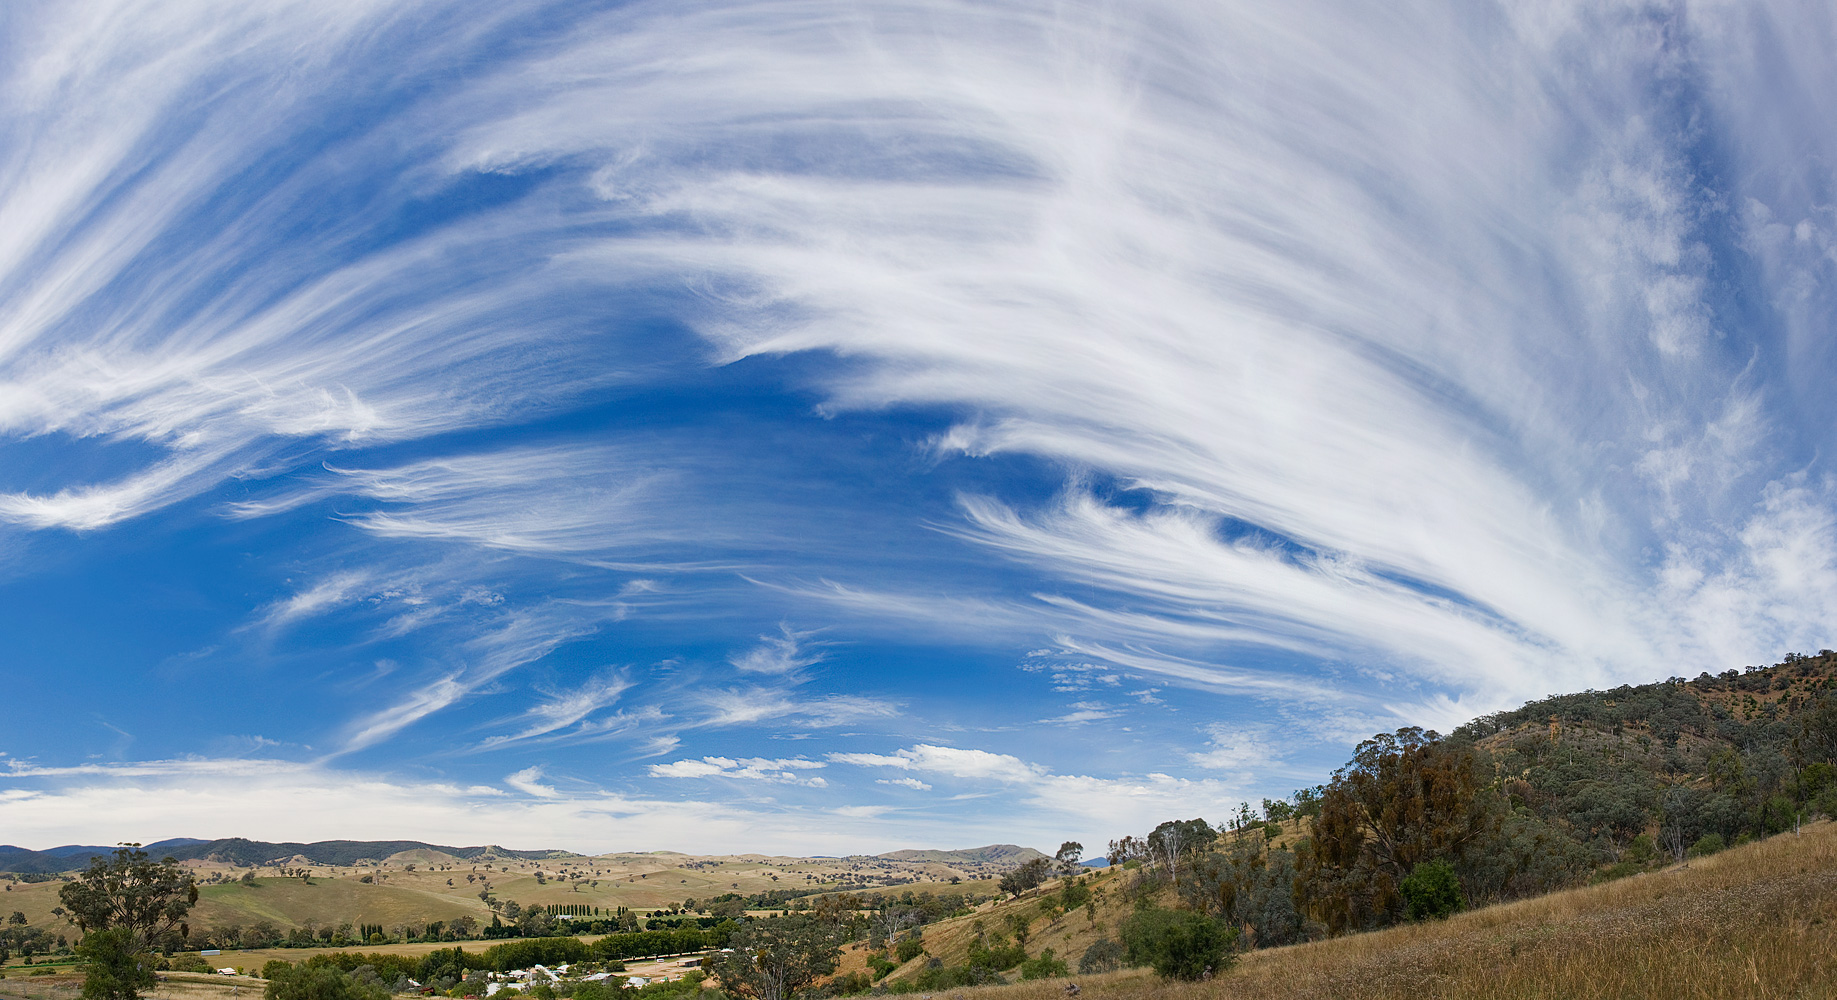
\includegraphics[height=\paperheight]{clouds.jpg}
    };
  \end{tikzpicture}
\end{frame}

\begin{frame}{Haskell test}
  \begin{center}
    \footnotesize
    \code{code.hs}{1}{12}{haskell}
  \end{center}
\end{frame}

\begin{frame}\label{lastframe}
  Copyrighted stuff:
  https://en.wikipedia.org/wiki/File:Cirrus\_sky\_panorama.jpg \\
  http://www.wallpapervortex.com/wallpaper-15684\_1\_other\_wallpapers\_my\_little\_pony.html
\end{frame}